
\begin{multicols}{2}
	{\normalsize Fonte: \href{https://pt.wikipedia.org/wiki/Osso_de_Ishango}{https://pt.wikipedia.org/wiki/Osso\_de\_Ishango}}
	
	{\large Paleolítico Superior ($\sim$20 000 - 18 000 a.C.)
	
	É um longo osso castanho (a fíbula de um babuíno) com um pedaço de quartzo afiado incrustado em uma ponta, que talvez fosse utilizado para gravar ou escrever.
}
\vfill\null
\columnbreak	

	\begin{center}
		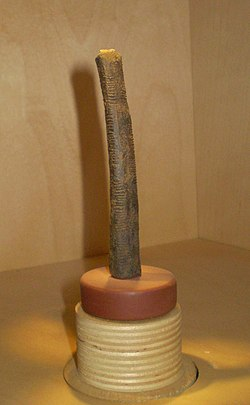
\includegraphics[height=.75\textheight]{./IMG/Os_d'Ishango_IRSNB.JPG}
	\end{center}


\begin{center}
	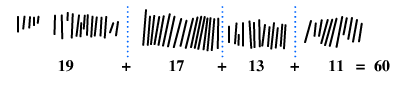
\includegraphics[width=\linewidth]{./IMG/IshangoColumnA.png}

	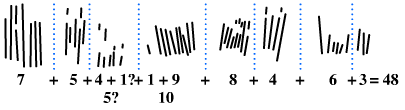
\includegraphics[width=\linewidth]{./IMG/IshangoColumnB.png}

	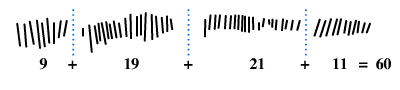
\includegraphics[width=\linewidth]{./IMG/IshangoColumnC.png}
\end{center}

\vfill
\columnbreak

	{\large Cogitou-se a princípio que era utilizado para realizar contagens, porque há uma série de traços talhados, divididos em três colunas, ao longo de todo o comprimento da ferramenta.}


\vfill\null
\pagebreak
\end{multicols}


